\section{OSI Model}

The Open Systems Interconnection (OSI) model describes
communications from the physical implementation of
transmitting bits across a transmission medium to the
highest-level representation of data of a distributed
application. Each layer has well-defined functions and
semantics and serves a class of functionality to the
layer above it and is served by the layer below it.

\subsection{Physical}

The realm of electrical and computer engineers.
Deals with converting between digital and analog signals or
electrical and optical signals. Beyond the purview of
this course.

\subsection{Data Link}
The data link layer runs on top of the physical layer.
It transfers data between nodes on a network segment
across the physical layer. Whereas the internet as a whole
runs on a global standard (IP) to allow subnetworks to
communicate, the data link layer allows autonomy
within each local area network (LAN).
Each LAN can run its own network
protocol for communication within LAN,
e.g., Ethernet, Wi-Fi, 5G, CSMA, Sonet, etc.
The data link layers handles addressing,
destination discovery, forwarding, and routing within
a local network. We will study data link layer mechanisms in the
context of the most popular data link layer protocol
called “Ethernet”
Ethernet is an example of a wired data link layer protocol,
i.e., nodes are connected using physical cables
\marginnote{
    Another very popular data link layer protocol is Wi-Fi,
    which is an example of a wireless data link layer protocol.
    Wi-Fi is not covered in this class}

\paragraph{MAC Addresses}

All network devices are connected to the network via a
“Network Interface” or “Port”. A network interface can be
“physical” (wired or wireless), such as an actual connection
on a server in some closet, or it can be “virtual”, i.e., a
piece of software emulating a network interface.
Each network interface, physical or virtual, has a Media Access
Control (MAC) address. MAC addresses are 48 bits or 6 bytes long and
typically represented in hexadecimal format, e.g., \texttt{ab:00:05:2c:e4:34}.
MAC address of each interface within a given network must be unique,
but MAC addresses are not necessarily globally unique.

There are three ways to transmit information from a sender to a
recipient:
\begin{itemize}
    \item Unicast: one-to-one transmission
    \item Multicast: many-to-many transmission
    \item Broadcast: one-to-all transmission
\end{itemize}

Naive implementations of
broadcast might have the sender send its packet to every of the
$N-1$ hosts in the network, but a more efficient implementation
is to send the packet to the router and have it send it out
to everyone else.
A special destination MAC address of \texttt{ff:ff:ff:ff:ff:ff} is used
to indicate a broadcast packet.

To see the list of interfaces on your computer, run the following
command in the terminal: \texttt{ifconfig} (mac/Linux) or
\texttt{ipconfig} (Windows).

In Ethernet, the Ethernet data (payload) and header is carried in an “Ethernet Frame”.
The structure of an Ethernet frame is as follows:
All Ethernet packets start with a “Preamble” - 7 bytes of alternating 1s and 0s
used for clock synchronization between sender and receiver.
This is followed by the Start Frame Delimiter (SFD), the one byte
\texttt{10101011}, then the destination MAX address, 6 bytes, and
then the source MAC address, 6 bytes. These are followed by the
Ethernet type, 2 bytes, which specifies the protocol carried in
the payload of the packet (e.g. IP), and finally the data itself.
The data has a minimum size of 46 bytes and a maximum size specified
by the Maximum Transmission Unit (MTU), which is configurable.
Everything is capped off with a Frame Check Sequence (FCS) of
four bytes, used for bit error correction and detection, and an
Inter Packet Gap (IPG), which is minimum 12 bytes of all 0s.

\paragraph{ARP}

The Address Resolution Protocol (ARP) is used to get the MAC
address of a destination host
within the same local network as the source host. It
assumes you know the IP address of the destination host.
Each host maintains a local table called ARP table
which stores a mapping between an IP address and MAC address,
as in Figure \ref{fig:arptable}.
\begin{figure}
    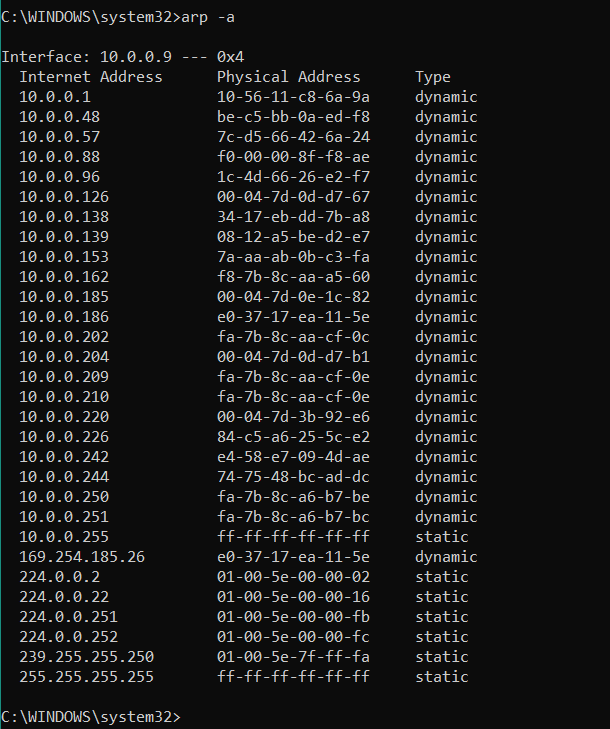
\includegraphics{images/arptable.png}
    \caption{ARP Table}
    \label{fig:arptable}
\end{figure}
Run \texttt{arp -a} on mac/Linux to view the table,
If the entry is found in the table, done!
Else run ARP to get the MAC address.

The ARP protocol has three stages. Say a host needs the MAC address
of some machine that it has the IP address of. The host broadcasts
an Ethernet frame with an ARP request. The structure of an ARP request
is as follows:
\begin{enumerate}
    \item Hardware type
    \item Protocol type
    \item Hardware size
    \item Protocol size
    \item Opcode
    \item Sender MAC
    \item Target MAC (all 0s)
    \item Target IP
\end{enumerate}

Everyone on a local network gets the
request. If the target IP matches the host
IP, it sends an ARP reply packet.

The structure of an ARP reply is
\begin{enumerate}
    \item Hardware type
    \item Protocol type
    \item Hardware size
    \item Protocol size
    \item Opcode
    \item Sender MAC
    \item Sender IP
    \item Target MAC
    \item Target IP
\end{enumerate}

On getting the ARP reply packet back,
the originating host updates its ARP
table with a new mapping from the target
IP address to target MAC address.

There are two ways of connecting nodes.
\begin{itemize}
    \item Shared medium: All nodes connected via single common medium,
          such as a wire or space itself in the case of wireless transmissions.
          Each packet sent over the shared medium is received by each host.
          On receiving a packet, a host checks destination MAC address
          and discards if it does not match host's MAC address
    \item Point-to-Point: Dedicated pairwise connections.
\end{itemize}

An issue with shared medium is that there can be collisions.
The solutions are somewhat technology-dependent, so
we will discuss the solution in the context of
Broadcast Ethernet where the shared medium is a wire.

There are two classes of techniques:
\begin{itemize}
    \item Reservation, including frequency division multiple access (FDMA) and
          time division multiple access (TDMA)
    \item On-demand, including random access
\end{itemize}

In FDMA, we divide the medium into frequencies.
Each source is assigned a subset of frequencies and
sends on its assigned frequency. With TDMA, divide time
into time slots. Each source is assigned a subset of time slots and
sends on its assigned time slot. The benefit of these
strategies is that we avoid collision.
However, if source is idle, then its frequency/time slot is wasted.
In FDMA, noise interference may cause disruption
In TDMA, if source has data to send, can't send immediately,
wait for its slot. TDMA also requires clocks of all hosts to be
synchronized.

With random access, when a source has a packet to send,
it sends it out. Unfortunately this leads to corruption
when two packets collide. T

here are methods to detect mitigate
corruption. One is to have the sender keep listening to
the medium while transmitting. If sender senses collision
(e.g., excess current on the wire), it aborts transmission
and broadcasts a “Jam” signal. A Jam signal is a random
32-bit signal that ensures that all receiving nodes fail
CRC checksum and discard the frame. The sender then
waits for a random time and resends to avoid instantly
colliding again.

Another method to mitigate corruption is
Carrier Sense Multiple Access (CSMA). In CSMA, the sender
listens to the shared medium before transmitting.
If idle, it starts transmitting. If busy, it waits.
This does not eliminate collision because of non-zero
signal propagation delay.

Together this collision detection and CSMA are called CSMA/CD.
CSMA listens to the medium and waits for it to be idle before
transmitting. CD sends a Jam signal if a collision is detected.
For re-transmission, most implementations use random
exponential backoff.
After a packet collision, sender tries to re-transmit
packet after a wait time. After $k$ collisions for a packet,
choose wait time randomly from $\{0,...,2^k - 1\}$ time slots.
$k$ resets to 0 after a packet transmission succeeds. This
gives exponentially increasing wait time with each attempt, but
also exponentially larger success probability with each attempt.

CSMA/CD does not scale to large number of hosts.
It gets a higher collision rate, wastes more bandwidth
re-transmitting the same packets, and has high and unpredictable
delay due to variable back-off times.
In practice, shared LANs don't have more than 1000 hosts
Another issue is that CSMA/CD assumes hosts send packets intermittently.
If everyone is sending steadily at all times there will be
more collisions. In addition, for CD to work, the sender must be
able to detect collision (if it
happens) before it is finished transmitting the entire packet.
If that's not true then the sender might have sent out multiple
packets before receiving the Jam signal. On re-transmit,
some receivers might receive duplicate packets. This
imposes a constraint on the
minimum packet size or maximum network length.
At high bandwidth, CSMA/CD requires either
large min packet size (wasted bandwidth when less data to send!)
or small network length.

So how do we overcome the scalability issue?
With a point-to-point forwarding device, as in Figure
\ref{fig:forwardingdevice}.
\begin{figure}
    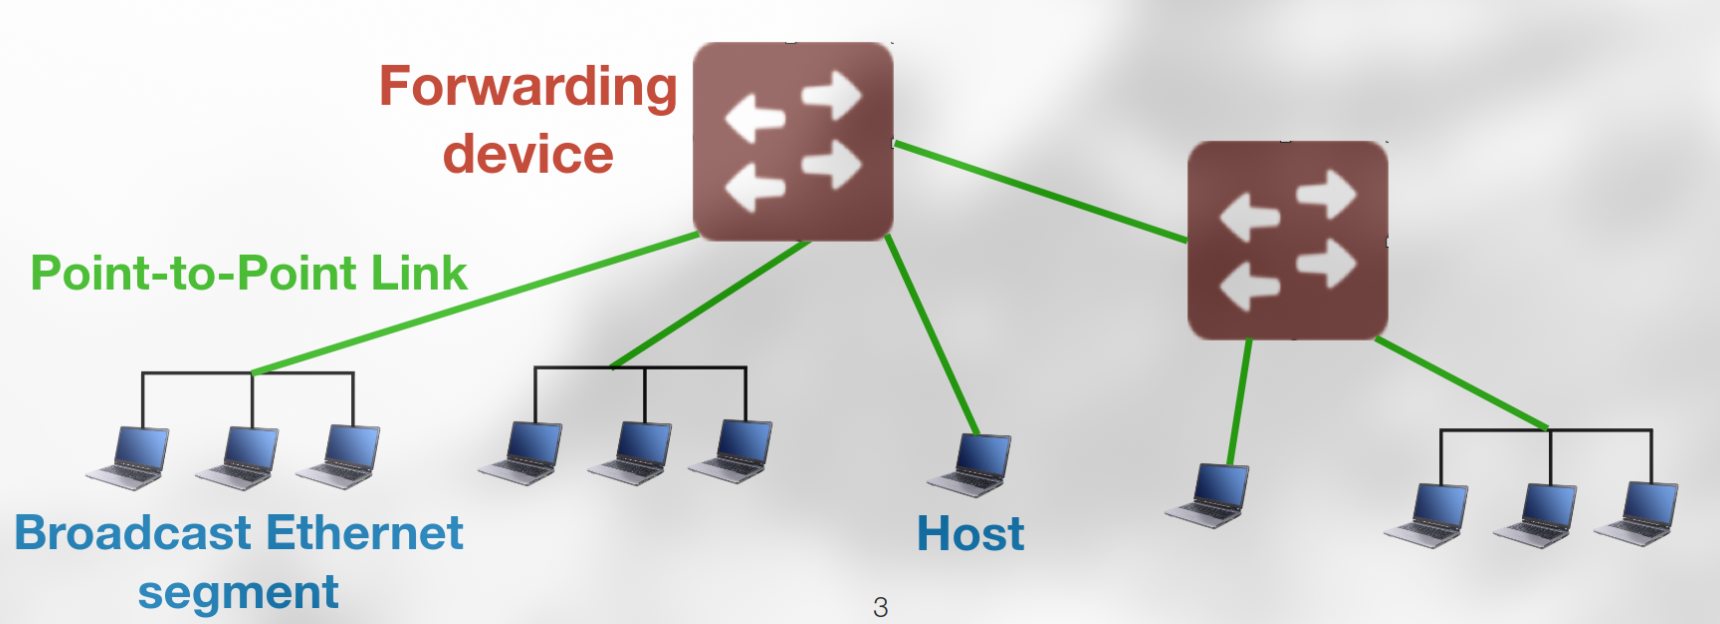
\includegraphics{images/forwarding-device.png}
    \caption{Forwarding Device}
    \label{fig:forwardingdevice}
\end{figure}
A point-to-point forwarding device
typically comprises multiple ports (or network interfaces).
Each port connects to a single host or multiple hosts sharing a
medium or some other forwarding device, using point-to-point links.
It forwards packets received on one port out on some other port.

There are three layers for forwarding devices, although a given
device can function at multiple layers:
\begin{itemize}
    \item Layer 1: operates at Physical layer, i.e.,
          forwards using physical layer
          packet header fields. Example: a Hub
    \item Layer 2: operates at Data Link layer, i.e.,
          forwards using Data Link layer
          packet header fields (e.g., using destination MAC address).
          Example: a bridge or switch.
    \item operates at Network layer, i.e., forwards using Network layer
          packet header fields (e.g., using destination IP address).
          Example: a router.
\end{itemize}

\paragraph{Layer 1} A layer 1 device, the hub, is the simplest possible
forwarding device. It broadcasts frame received on a given port to all
other ports except the port the frame was received on.
Physical layer headers contain no address information, so broadcast is
the only option. Typically a hub connects multiple Broadcast Ethernet segments.
and helps extend Broadcast Ethernet to larger distance
by providing signal amplification and signal re-generation. Nobody really uses
hubs these days because they just create bigger Ethernet segments,
which still have collisions.

\paragraph{Layer 2} The simplest layer 2 device is a bridge. It understands
MAC addresses and creates two half-duplex point-to-point connections
between its two ports. A generalized version of the bridge, the switch,
is the most commonly used device. A switch is a multi-port bridge, i.e.,
has $N > 2$ ports. It creates $N$ half-duplex point-to-point connections
(a \emph{matching}) between input and output ports using a crossbar,
which is just a bunch of wires going between input and output ports.
A matching is a bipartite graph
where every edge has a unique endpoint.

An algorithm
called iSLIP decides the matching configuration.
iSLIP looks at the current \emph{demand}, i.e., for each input packet
what is the output port.
iSLIP then configures the crossbar to create the matching that satisfies
the most demands.
It repeats the above two steps iteratively till all demands are satisfied.

Ethernet running inside a switch is called “Switched Ethernet”.
Modern Ethernet LANs run Switched Ethernet
instead of Broadcast Ethernet.

In switched ethernet, each switch maintains a “Forwarding Table”
Which keeps track of which hosts are reachable via each output port.
For the network in Figure \ref{fig:switchedethernetnetwork}, the
forwarding table is given by the table below.
\begin{figure}
    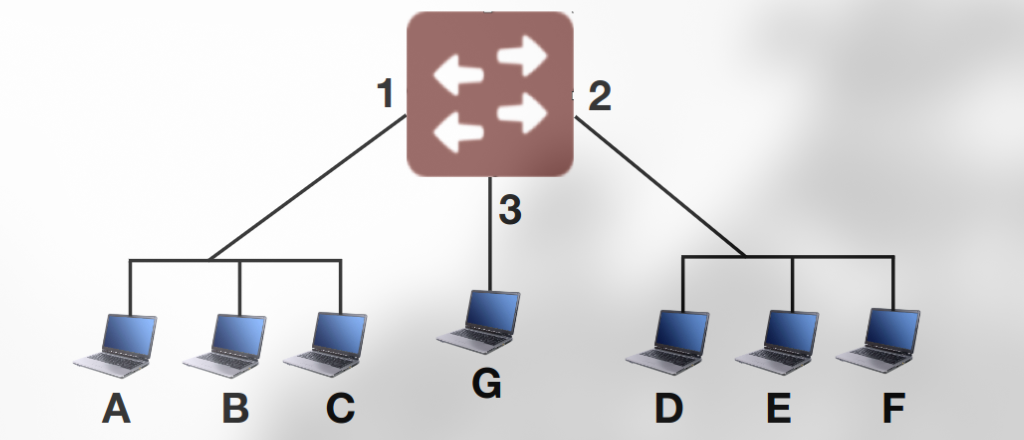
\includegraphics{images/switchedethernetnetwork.png}
    \caption{Switched Ethernet Network}
    \label{fig:switchedethernetnetwork}
\end{figure}

\begin{table}[h]
    \centering
    \begin{tabular}{|c|c|}
        \hline
        \textbf{Destination MAC Address} & \textbf{Output Port} \\ \hline
        A.mac                            & 1                    \\ \hline
        B.mac                            & 1                    \\ \hline
        C.mac                            & 1                    \\ \hline
        D.mac                            & 2                    \\ \hline
        E.mac                            & 2                    \\ \hline
        F.mac                            & 2                    \\ \hline
        G.mac                            & 3                    \\ \hline
    \end{tabular}
\end{table}

To populate the forwarding table, use the following algorithm.
When a switch receives a frame on port p, it checks the source
MAC address in the frame. Let it be $s$.
The switch learns that host with MAC address $s$ is reachable via port $p$,
so it adds the entry $<s, p>$ to its forwarding table.
If a switch never receives a frame sourced from a host, it
will never learn which port the host is reachable on.

The way MAC forwarding works is that, upon receiving a frame with destination
MAC $d$ and if \texttt{d = ff:ff:ff:ff:ff:ff}, copy and send frame on every
port except the port on which the frame was received on. This is a broadcast.
If $d$ is not \texttt{ff:ff:ff:ff:ff:ff}, then check the forwarding table
for an entry $<d, p>$. If entry $<d, p>$ exists, then if $p$ is same as the
port on which frame was received, then drop the frame. Otherwise send frame
out on port $p$. Else if no entry corresponding to $d$ exists, the switch
copies and sends frame on every port except the port on
which the frame was received on, again a broadcast. If there is a loop
in the network graph, then a broadcast packet can cause infinite loops
and consume all resources in a broadcast storm. The way to avoid this
is to structure networks as spanning trees with no loops. Doing this
in a distributed way is extremely complex, and MAC learning by itself
can't handle finding a route with no loops.

Luckily, the \emph{Spanning Tree Protocol} (STP) extends MAC learning
to detect and remove loops from the graph. The task of STP is, given
a network of switches and end hosts, to create a graph where vertices
represent switches/hosts and edges represent links, then to remove all
loops from the graph. The way STP accomplishes this is by, unsurprisingly,
building a spanning tree, a subgraph that includes all vertices but no
cycles. In a spanning tree there is exactly one path between vertex pairs,
which means there will be no loops.

Unfortunately, no single switch has full view of the graph,  so
we need to build the spanning tree in a distributed manner. In STP,
switches exchange messages to build the spanning tree. These messages
are carried in special packets called \emph{control packets}. These
packets are distinct from normal Ethernet packets and have STP-specific
info. Control packets in STP are only exchanged between directly connected
neighbor switches and are never forwarded beyond that. Control packets
are only used for STP and are not used for MAC learning and forwarding.

STP has three steps:
\begin{enumerate}
    \item Pick a root: pick the switch with the smallest MAC address.
    \item Compute the smallest cost path to the root. For each switch,
          calculate the smallest cost path to the root. Where there are
          multiple smallest cost paths to the root, choose the path via
          neighbor switch with the smaller MAC address.
    \item Make links not on any smallest cost path "inactive". For link A-B,
          if neither A nor B uses it on its smallest cost path, then it's "inactive".
          Switches do not forward any data packets on that link and ignore
          any received data packets on that link. However, continue to send
          and receive control packets on "inactive" links to handle failures where
          they may need to be reactivated.
\end{enumerate}

Each switch maintains a view $(R, \text{cost}(X, R), X, H)$.
$R$ is the current root according to $X$. $\text{cost}(X, R)$
is the cost from $X$ to $R$. $H$ is the next hop neighbor via
which $X$ reaches $R$.

A control packet from neighbor $X$ to $Y$ carries $X$'s current
view, $(R, \text{cost}(X, R), X, H)$ where $X$ is proposing $R$
as root and advertising a cost of $\text{cost}(X, R)$ from $X$
to $R$ via neighbor switch $H$ (next hop to root from $X$).
The algorithm converges when no switch view changes on
receipt of a control packet.

\begin{lstlisting}
    // propose this switch as root
    send (X, 0, X, X) to all neighbors

    // on recieve (R, cost(Y, R), Y, H)
    // from neighbor Y
    when control packet recieved
        if advertisement from current next hop to root
            if R < X
                view = (R, cost(X, Y) + cost(Y, R), X, Y)
        else 
            // also update if same root, same cost, smaller MAC
            if smaller root or cost path advertised
                update
            
\end{lstlisting}

The protocol must react to failures and link cost changes in
the network. Switches, including the root, can fail. Links can
fail or their cost can change.
Each switch $X$ tracks the status of
its current next hop $H$ and link
$X-H$. On detecting failure of $X$ or
$X-H$, $X$ updates its view to
$(X, 0, X, X)$.
Each switch $X$
periodically sends its view $R, \text{cost}(X, R), X, H)$
to all its neighbors. This is
needed for convergence under certain
failure scenarios and makes STP robust
to control packet corruption and loss.

The final Spanning Tree Protocol
operates as follows: Initially,
each switch proposes itself as the root,
setting its view to $(X, 0, X, X)$ and
sending a control packet $(X, 0, X, X)$
to all neighbors. Upon detecting a failure
of its next hop ($H$) or the link $X-H$,
switch $X$ updates its view to $(X, 0, X, X)$
and advertises this new view to all neighbors.
Each switch periodically sends its current
view $(R, \text{cost}(X, R), X, H)$ to all neighbors.
When receiving a control packet $(R, \text{cost}(Y, R), Y, H)$
from neighbor $Y$, switch $X$ updates its view according to
predefined cases (Case 0, 1, and 2). If $X$'s view changes,
it sends its new view in a control packet to all neighbors.
Additionally, $X$ checks the next hop of neighbor $Y$ each
time a control packet is received from $Y$. A link $X-Y$ is
made "inactive" if and only if the next hop of $X$ is not $Y$
and the next hop of $Y$ ($H$) is not $X$, at which point $X$
stops forwarding data packets on that link, removes related
entries from the forwarding table, and ignores data packets
received on $X-Y$ for MAC learning and forwarding. The
algorithm converges when no switch updates its view upon
receiving a control packet.

\subsection{Network}
The network layer runs on top of runs on top of the
“best-effort” local area delivery service data link
layer. While the data link layer allows
information to be relayed within a local
network, the network layer connects
different local networks. As with all
layers, we must solve the problems
of addressing, destination discovery,
forwarding, and routing. The problems
are the same, but the scale is different
so the solutions must be different.
The IP address replaces the MAC
address, IP forwarding replaces MAC
forwarding, network routing protocols
(DV, LS, BGP) replace MAC learning
with STP, and destination discovery
with DNS replaces ARP.

As the most popular protocol with the
data link layer is Ethernet, the most
popular protocol with the network
layer is \emph{internet protocol}
(IP).

While the MAC tells the identity
of the host, the IP address tells
the location of the host. The MAC
address of a host does not change
(in most cases), and so can provide
host-based services such as allowing
access to a network service to an
authorized computer, regardless of
the location of a computer. IP
addresses allow reaching distant
devices. IP address do this by
constructing a hierarchy so that
each router only needs to store
the IP address of the networks
immediately above and below it
in the network hierarchy.

STP doesn't work as a routing
protocol at the network since
it finds the shortest path to
the root and not the destinations.
STP also has higher latency and
wasted bandwidth. The pros of
simplicity and quick convergence
outweigh the cons of higher
latency and wasted bandwidth
for small networks, but not for
large. With network routing
protocols, each router finds
the shortest path to each
destination, and there is no
root. The pros are better
latency and better bandwidth
utilization, but at the cost
of higher complexity and
taking longer to converge. The
pros outweigh the cons for
large networks.

ARP doesn't work for large networks
because it requires broadcast
requests to every host on the
network. DNS requires dedicated
infrastructure and extra mechanisms
for fault tolerance, but doesn't
require broadcasts, which is
good for large networks.

IP is really the only protocol for the network layer.
This is in stark contrast to every other layer, which
have a proliferation. In this class we'll focus on IPv4
instead of the newer IPv6. In IPv4,
IP addresses have 32 bits and are
represented as \texttt{X.X.X.X} where
\texttt{X} is an 8-bit decimal, e.g.
\texttt{192.168.3.29}.

Hosts within a subnet share the same
subnet address prefix. So perhaps
devices in the same subnet have IP
addresses \texttt{X.X.X.92},
\texttt{X.X.X.23}, and \texttt{X.X.X.01}.
Any hierarchy can be encoded in the IP
address; perhaps the first $n_0$ bits
correspond to a given country, the next
$n_1$ to an internet provider in that
country, the next $n_2$ to an organization,
the next $n_3$ to a location, etc.

We use a subnet mask to extract the
subnet address from the IP address.
The subnet mask a 32 bit long series
of 1s followed by a series of 0s.
For example, \texttt{255.255.240.0}
is 20 1s followed by 12 0s. The subnet
address is the bitwise AND of the
IP address and subnet mask. For the
previous example, with an IP address
of \texttt{192.168.3.29} the subnet
address would be
\texttt{192.168.3.29 \& 255.255.240.0 = 192.168.0.0}.

Under classful addressing, IP addresses
are divided into a set of classes.
Each class has $n$ bits statically
allocated for a subnet address and the
remaining $32-n$ bits are for the
host identifier. Depending on the
value of $n$, there are three
popular classes.
\begin{itemize}
    \item A: $n=8$, MSB \texttt{0}, 8 subnet bits, 24 host bits, 128 subnets, $2^24$ hosts.
    \item B: $n=16$, MSB \texttt{10}, 16 subnet bits, 16 host bits, 16K subnets, $2^16$ hosts.
    \item C: $n=24$, MSB \texttt{110}, 24 subnet bits, 8 host bits, 2M subnets, $2^8$ hosts.
\end{itemize}
The issue with classful IP addressing is that the division of bits between subnet
and host addresses are not flexible. So to support 129 subnets one should need
only 8 bits for subnet address, but with classful IP addressing, one will need a B
class address, which uses 16 bits for the subnet address, wasting 8 bits.

The more widely implemented method is called \emph{Classless Inter-Domain Routing}
(CIDR). CIDR allows a flexible number of bits to be allocated for the subnet
address. In CIDR notation, a subnet address is represented as \texttt{X.X.X.X/n}.
The first \texttt{n} bits are allocated for the subnet address, meaning the subnet can
support $2^{32-n}$ IP addresses. For example, the subnet address \texttt{128.32.0.0/11}
can support $2^21$ IP addresses in the range \texttt{128.32.0.0} to \texttt{128.63.255.255}.

Hosts have two options for configuring their IP addresses. They can either do it manually
and pick whatever IP address they want, or they can implement the \emph{Dynamic Host
    Configuration Protocol} (DHCP) and have an IP automatically assigned to them. The way
this works is that DHCP typically runs on the router and maintains a pool of allowed
IP addresses for a network, and when a host connects, the router assigns it an IP
address.

There are public IP address, used for routing over the internet, and private IP
addresses, for communication within a private network. Public IP addresses are
assigned by the Internet Corporation for Assigned Names and Numbers (ICANN).
ICANN allocates large IP blocks to regional internet registries, e.g. the middle East,
Europe, central Asia. Each internet registry allocates address blocks to large \emph{internet
    service providers} (ISPs) within that region. The ISP allocates addresses to individuals
and smaller institutions. For instance, ICANN allocates some \texttt{X.0.0.0/8} addresses
to ARIN, which allocates one /8 address to AT\&T, which allocates
one /16 address to Purdue, which allocates one /24 address to ECE, which gives your
computer an IP.

Hosts over the internet need a unique public IP address for correct routing, but
there are only $2^{32} \approx 4000000000$ unique IPv4 addresses. The number of
modern devices would exhaust this very quickly if not for private IP addressing.

Private IP addresses can be used for communication only within a private network,
and packets with private IP addresses as destinations are dropped by public internet
routers. Hosts in different private networks can have the same private IP address,
which helps with the problem of IPv4 address exhaustion. The reserved private IP
address ranges are
\begin{itemize}
    \item \texttt{10.0.0.0/8} (\texttt{10.0.0.0} to \texttt{10.255.255.255})
    \item \texttt{172.16.0.0/12} (\texttt{172.16.0.0} to \texttt{172.31.255.255})
    \item \texttt{192.168.0.0/16} (\texttt{192.168.0.0} to \texttt{192.168.255.255})
\end{itemize}

Network Address Translation (NAT)
enables hosts on private networks to
communicate with hosts on the Internet.
A NAT device sits at the boundary of a private network and the
public Internet (typically implemented inside a gateway router)
and manages a pool of public IP addresses allocated to the
private network.
When a host from the private network wants to send an IP packet
to a host in public Internet, NAT picks a public IP from the pool and
re-writes the (private) source IP in the packet with public IP.
It also stores the private IP to public IP mapping in a table to re-
translate the (public) destination IP of an incoming reply packet
from the Internet with the corresponding private IP.
On its own, this doesn't help with the problem of IP address exhaustion.
Ideally, NAT should share a small number of public IPs
between a large number of private hosts. This is done with IP
masquerading.
\marginnote{
    IP masquerading is also called Network Address and Port
    Translation (NAPT) or Port Address Translation (PAT).
}
With IP masquerading, a single public IP is mapped to multiple
hosts in a private network.
Hosts mapped to the same public IP are assigned different
port numbers to distinguish them from one another.
A port number is 16 bits, meaning one can support $2^16$ hosts
using a single public IP address.

This comes with a cost. NAT destroys universal end-to-end
reachability of hosts on the Internet. A host on public
Internet cannot initiate direct communication to a
host with a private IP address. Applications that carry IP
address in the payload of the application data
(e.g., HTTP) generally do not work across a private-public
network boundary.
\marginnote{
    Some NAT devices inspect the payload of widely used application layer
    protocols, and if an IP address is detected, they do the translation.
}

An IP packet, also called an IP datagram, is the fundamental unit of data exchanged at the network layer. Each packet consists of a header and a payload. The header contains all necessary information for routing and delivery, while the payload carries the data from the transport layer (e.g., TCP or UDP segment).

The structure of an IPv4 packet is as follows:

\begin{itemize}
    \item \textbf{Version (4 bits)}: Specifies the IP version. For IPv4, this value is \texttt{4}.
    \item \textbf{Header Length (4 bits)}: Specifies the length of the header in 32-bit words. The minimum value is \texttt{5}, corresponding to 20 bytes.
    \item \textbf{Type of Service (8 bits)}: Indicates the priority and quality of service desired for the packet, such as low delay or high reliability.
    \item \textbf{Total Length (16 bits)}: The total size of the IP packet in bytes, including both header and payload. The maximum value is \texttt{65535}.
    \item \textbf{Identification (16 bits)}: A unique identifier assigned to each packet so fragments of the same packet can be reassembled.
    \item \textbf{Flags (3 bits)}: Controls or identifies fragments. The most important flag is the "More Fragments" bit, which is set if more fragments follow.
    \item \textbf{Fragment Offset (13 bits)}: Indicates the position of the fragment relative to the start of the original packet.
    \item \textbf{Time to Live (TTL) (8 bits)}: The maximum number of hops (routers) the packet can traverse before being discarded. Each router decrements the TTL by one; if it reaches zero, the packet is dropped.
    \item \textbf{Protocol (8 bits)}: Specifies the protocol carried in the payload, such as \texttt{6} for TCP or \texttt{17} for UDP.
    \item \textbf{Header Checksum (16 bits)}: Used for error detection on the header only. Each router verifies and recomputes it.
    \item \textbf{Source IP Address (32 bits)}: The IP address of the originating host.
    \item \textbf{Destination IP Address (32 bits)}: The IP address of the intended recipient.
    \item \textbf{Options (variable length)}: Optional field used for features such as record route, timestamp, or security.
    \item \textbf{Padding (variable length)}: Added to ensure the header length is a multiple of 32 bits.
    \item \textbf{Data (variable length)}: The payload, usually a transport-layer segment such as TCP or UDP data.
\end{itemize}

A typical IPv4 header without options is 20 bytes long.
The payload size depends on the Maximum Transmission Unit
(MTU) of the underlying data link layer. If an IP packet
is larger than the MTU, it is divided into smaller fragments.
Each fragment is then reassembled by the destination host
using the Identification, Flags, and Fragment Offset fields.

IP provides a best-effort delivery service, meaning it does
not guarantee reliability, ordering, or data integrity beyond
basic error detection on the header. These functions are
handled by higher-layer protocols such as TCP in the transport layer.

Network routing protocols are used to populate the routing tables.
They calculate the best path from each router to all other routers/
hosts, unlike STP which calculates the best path from each switch
to a root switch.

Networking routing protocols come in two flavors: \emph{distributed path}
computation and \emph{distributed topology} computation.

Distributed path computation is similar to STP in that each router computes paths
using a distributed algorithm, oblivious of network topology. The distance vector (DV)
and border gateway (BG) algorithms fall into this category.

The distance vector algorithm is a distributed version of the Bellman-Ford algorithm that
calculates the least cost path from each router to all the $n$ routers and hosts.
Each router maintains a vector of views of its least cost path to all other routers and
hosts. It shares its vector with all its neighbor routers and updates the vector and
receiving vectors from its neighbors.
The most popular distance vector implementation is the \emph{routing information protocol}
(RIP).

DV does not prevent loops under all scenarios. We mitigate this with
split horizon, which dictates that if a router gets a vector that states
the next hop to a destination is itself, to drop the vector. This prevents
loops involving two routers, but cannot prevent loops of three or more.
To detect and remove all loops, set the \emph{max infinity counter} to
some value larger than the largest path cost in the network. When the cost
to a destination reaches or exceeds infinity, the router detects count-to-infinity.
On detection, the router removes the destination entry from its routing
table or sets the next hop for the entry to NULL. This is used alongside
split horizon, which tries to prevent loops.

Distributed topology computer is when routers use a distributed algorithm to learn the
entire network graph. Each router runs a local path computation algorithm on the learned
graph. This category includes link state (LS).

In link state, each router runs a distributed algorithm to learn the global
network graph. It then runs a local computation to find the shortest paths
and populate its routing table. The most popular link state implementation is
Open Shortest Path First (OSPF).

Each router $X$ maintains a view of the global network graph $G$. Initially,
$G$ is empty. For each neighbor $Y$, $X$ adds link $X-Y$ and link cost
$\text{cost}(X, Y)$ to $G$. $X$ creates a control packet called a link state
announcement (LSA) and sends it to all neighbors. The LSA contains the list of
all neighbors of $X$ and the cost to neighbors, i.e. $(Y, \text{cost}(X, y))$.
On receiving node $Y$'s LSA $(Z, \text{cost}(Y, Z))$ $X$ updates its graph $G$
by adding or updating link $Y-Z$ and the corresponding link cost. $X$ then
broadcasts the received LSA on all ports except the port it arrived on.
Every time $G$ changes, $X$ reruns the route computation algorithm locally.
It computes the least cost path from itself to all other nodes by using, for
example, Dijkstra's algorithm.

LSAs are sent when a router learns of a change to a neighbor, like a neighbor
or link to neighbor failed, a neighbor was added, or a link cost to neighbor
changed. LSAs are also sent periodically to correct possible corruption of
previous LSA data or previous LSA packet drops.

LSA comes with a big problem. Suppose $X$ sent an LSA at time $t$ with neighbors
$\{W, Z\}$. At time $t + 2$, a new link $X-V$ is added and $X$ sends a new LSA
$\{W, Z, V\}$. At router $Y$, LSA $\{W, Z, V\}$ arrives before $\{W, Z\}$
because the new link allowed the LSA to be propagated faster. After $\{W, Z\}$
arrives, $Y$ will conclude that $X$ only has 2 neighbors. This wasn't an
issue with STP and DV, because control messages were only exchanged between
directly connected neighbors.

One way to mitigate this could be to include a timestamp with each LSA
sent, and for $Y$ to ignore LSAs from $X$ whose "sent" timestamp is older than
any LSA that $Y$ has already received. This is essentially what routers do.
Each router $X$ maintains a local sequence number $S_x$ and while generating
an $LSA$, the router includes the current value of $S_x$ in the LSA before
broadcasting. With each LSA broadcast $X$ increments $S_x$ by 1. Each
router also maintains a list of the highest sequence number that it has
received from each of the other routers. This prevents loops in all scenarios,
although there can be transient loops. While LS has not converged, loops
can still be formed. To handle these transient loops each IP packet contains
an 8-bit \emph{time-to-live} (TTL) field in the header. The sending host
initializes the TTL with some value. TTL is decremented by one by the
router at each hop. When TTL reaches 0, the packet is dropped by the
router. TTL is not a substitute for routing protocols because it does not
prevent packets from getting in a loop, only reduces the amount of time
a packet spends in a loop.

The key difference between DV and LS is that DV advertises your paths to
everyone to your neighbors, while LS advertises your paths to neighbors
to everyone.

Recall that the internet is a hierarchical network of networks.
An autonomous system (AS) or domain is a network under a single
administrative domain. Each AS is assigned a unique identifier.

Intra-domain routing refers to routing within an AS. Examples:
RIP (distance vector), OSPF (link state).

Inter-domain routing refers to routing between ASes. Example: border gateway
protocol (BGP).

We can't simply use DV or LS for inter-domain routing because ASes want freedom
to pick routes based on custom policy. This can't be expressed as a least cost path
like in DV or LS, but rather depends on the business relationship between
ASes.

There are three basic kinds of relationships between ASes.

\begin{itemize}
    \item Customer, e.g. Purdue is AT\&T's customer. The customer pays the provider.
    \item Provider, e.g. AT\&T is Purdue's provider.
    \item Peer, e.g. AT\&T and Verizon are peers. Peers don't pay each other.
          Peers exchange roughly equal levels of traffic.
\end{itemize}

A customer is multi-homing if it has multiple providers. Provider ASes connect
customer ASes to the rest of the Internet, and customer ASes
pay the provider ASes for this service. Peering is needed to connect ASes
at the top, which have no providers. These ASes are known as Tier 1 ASes and
include ISPs like AT\&T, Sprint, Verizon. Peering can also be done at lower
levels for various reasons, such as two top secret institutions not trusting
a provider and exchanging information directly.

To set up inter-domain routing, destinations are subnets. Nodes are ASes, and
the internals of each AS are hidden. Physical links between ASes are tagged
with the corresponding business relationship. Border gateway protocol (BGP) is
user for routing.

In BGP, each AS advertises to neighbor ASes its best paths to one or more
subnets. Each AS selects the "best" path(s) from the set of advertised paths
to a subnet destination.

BGP is inspired by distance vector. It has per-distance route advertisements to
its neighbors. There is no global learning of network topology. It's iterative
and uses distributed convergence to final paths. But, there are three key differences.

\begin{itemize}
    \item While distance vector shares the distance and next hop to a destination,
          BGP shares the entire path to a destination to enable ASes to apply more
          complex policies. This makes loop detection trivial.
    \item BGP does not always select the shortest path.
    \item For policy reasons, an AS may choose not to advertise a route. Thus
          reliability is not guaranteed even if the graph is connected.
\end{itemize}

BGP policy is imposed in how route are selected and advertised. Selection
is which path to use to send data. It controls whether/how traffic leaves
the network. Advertisement is which path to advertise to other ASes. It
controls whether/how traffic enter the network. Traffic flows in the reverse
direction of the advertisement.

Typical selection policies are, in decreasing order of priority,
\begin{enumerate}
    \item Make or save money by preferring a path through the customer,
          then a path through a peer, then a path through a provider
    \item Maximize performance by selecting the shortest path
    \item Minimize use of network bandwidth aka "hot potato" routing
\end{enumerate}

The typical advertisement policy is Gao-Rexford advertisement policies,
whose goal is to avoid being transit when there is no monetary gain.
The customer advertises to providers, peers, and other customers. The
peer advertises to customers. The provider advertises to costumers.
The AS provides transit service to all its customer traffic, because that's
what customers pay for. It does not provide transit service between two
providers or peers, since these entities are not paying the AS.

\subsection{Transport}

\subsection{Application}


